\chapter{Background}

-Available spike analysis frameworks \\
-fieldtrip \\\
-elephant \\
-Why they are not sufficient \\
-problem with the relays? maybe windows updates 

 

-openMNGlab as a solution \\
-acquisition frameworks we need to handle \\
-Current status of openMNGlab, including Neo \\
-go into detail on different data acquisition softwares \\
-Dapsys, OpenEphys, Spike2 \\
-why does dapsys not work in the future \\

  

When deciding with which software to analyze the data there were multiple possibilities. 

There are the existing FieldTrip and Elephant tools, as well as the Software framework openMNGlab,  that all offer different analysis opportunities for electrophysiology data. 

Fieldtrip (fieldtriptoolboX.org) is a software developed at the Radboud University, Nijmegen, the Netherlands and offers a wide variety of analysis functions. The main problem with this software is its programming language. It is a MATLAB toolkit, however it would be preferred to use a software package in python or another programming language that slots better in the already existing structure within the chair for medical informatics. In addition to that it is not only speficied for spike trains software, dealing with MEG, EEG and iEEG analysis. 

Elephant (https://elephant.readthedocs.io/en/latest/index.html) is a python module which offers some high-level analysis functions for spike trains specifically. The main problem with this software is the lack of basic functionalities. It relies more on highly specified analysis tools that are not necessarily viable in our use-case. For the use in this thesis I want to start with the basic signal from the spikes, try out different quantifiers and look at the data from a fresh perspective. 

In the end I decided on using the software framework openMNGlab. It is a python framework being developed at the chair of medical informatics RWTH. It offers some basic import and analysis functionalities that are ideal for using in this Bachelor thesis. With this framework I can start from the beginning and develop my own quantifiers. 


\section{Data acquisition software} 
There are many different data acquisition software packages for electrophysiological data. 

\subsection{Spike2}
“Spike2 is a multi-channel continuous data acquisition and analysis package”( https://ced.co.uk/products/spkovin) produced by Cambridge electronic design limited. \\
-Used for the experiments I am analysing by Roberto \\
-records data in multiple channels \\
-channel for raw signal \\
-channel for mechanical force \\
-channel for event markers \\
-channel for temperature (not used by me) \\
-channel for comments (used for marking when chemicals are applied) \\
-spikes can be separated into own channels (done by experimenters) \\
-software offers a graphical representation of the data \\
-channels are separated \\
-was used for confirmation of what the data should output in terms of basic quantifiers \\
-can export csv files from the data \\
-has direct importer in openMNGlab \\

Spike2 is a data acquisition and analysis software produced by Cambridge electronic design limited. It is a flexible tool that can be used in a variety of different ways.

TODO: go into detail\\

\begin{figure}
	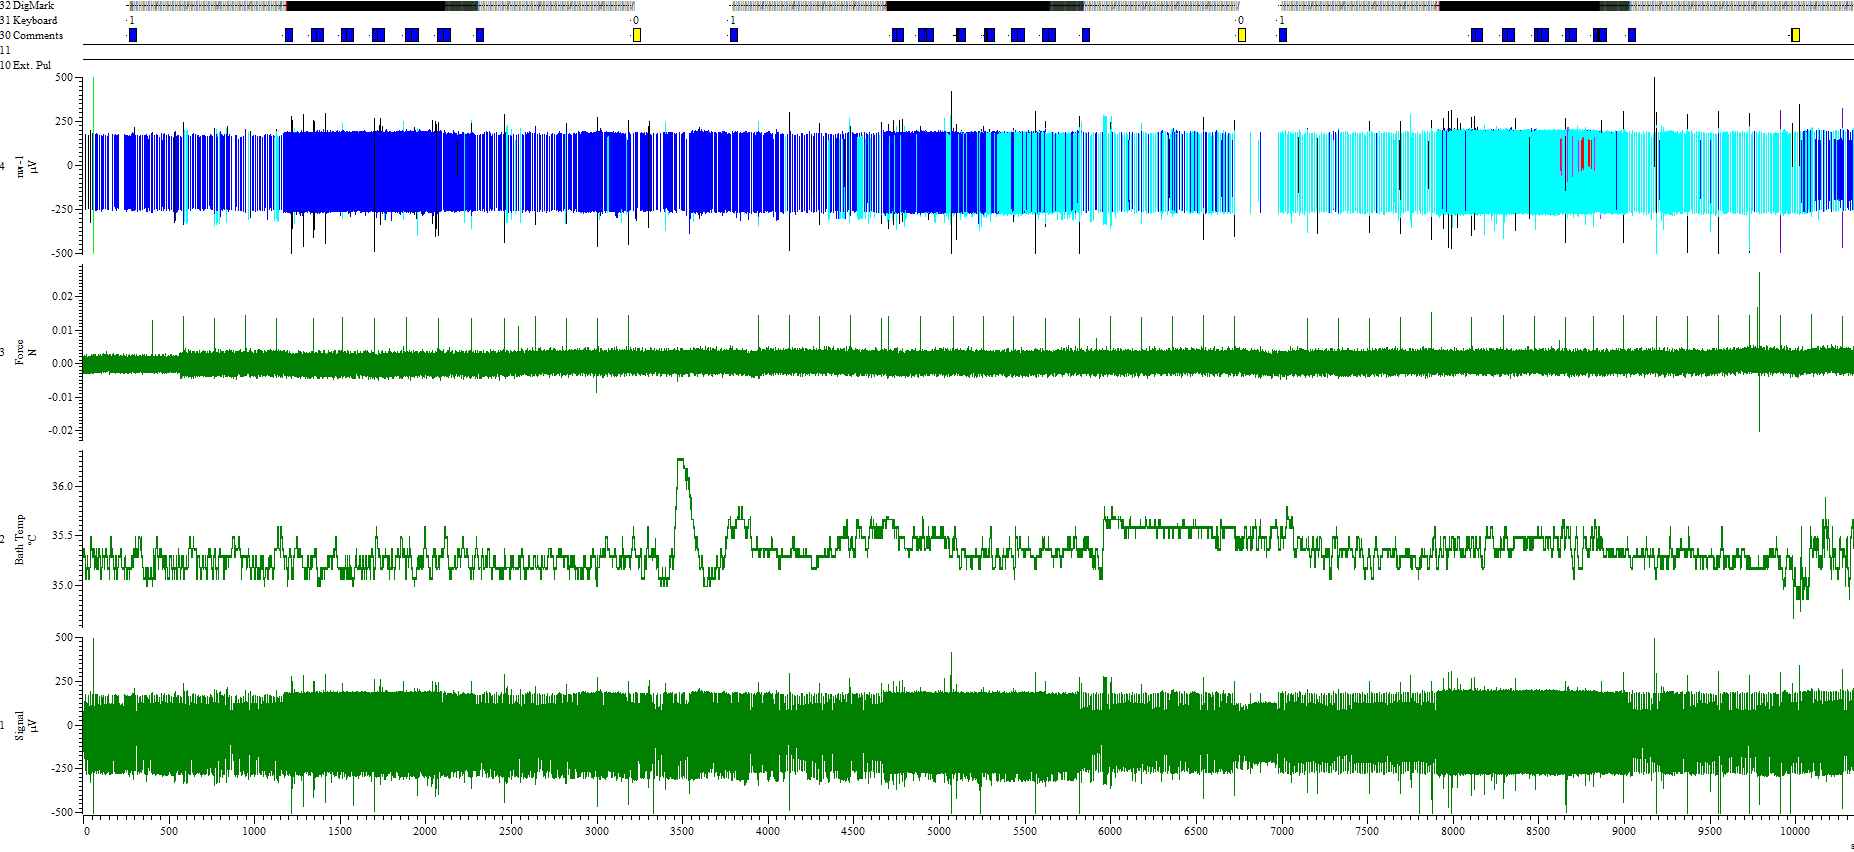
\includegraphics[width = \textwidth]{src/pic/Spike2_screenshot}
	\caption{Typical mechanically and electrically stimulated recording in Spike2}
	\label{fig:spike2}
\end{figure}

The software can record multiple channels simultaneously. An example screenshot from a recording can be seen in Figure~\ref{fig:spike2}. This depicts a typical recording used for analysis in this bachelor thesis. The recording contains data from nerve fibers of rat cranial dura mater. The nerve fibers were stimulated using a mechanoelectrostimulator applying electaical and mechanical stimulation. 

\begin{figure}
	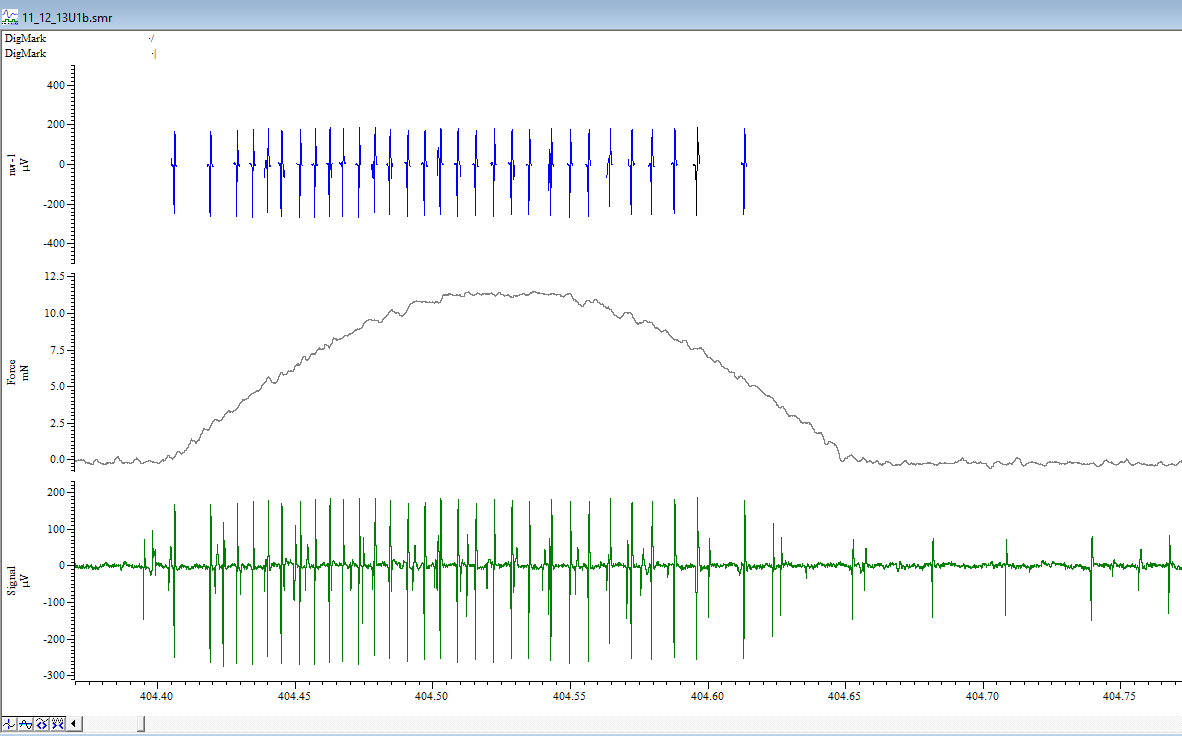
\includegraphics[width = \textwidth]{src/pic/Spike2_spike_train}
	\caption{A single spike train in spike2}
	\label{fig:spike_train}
\end{figure}

First of all it contains a channel for the recorded raw signal at the bottom. The next channel contains the temperature during the recording. In this example it fluctuates between 35°C and 36.5°C. In channel 3 we can observe the mechanical force that was applied to the nerve fibers. In Figure~\ref{fig:spike2} there are spikes in mechanical force whenever a mechanical stimulation occurs to evoke a spike train. For this experiment we want to collect the data of single nerve fibers. It is diffucult, to record just a single nerve fiber in vitro, however. This is why in this experiment spike templates are applied to the raw signal to filter out specific fibers. These filtered fibers are then displayed in channel 4, where only the action potentials of selected shapes are collected.\\
The topmost channel in Figure~\ref{fig:spike2} contains markers for the electrical and mechanical stimuli. Additionally there is a channel containing comments regarding the experiment. Comments can represent the experimental protocol and are filled in by the experimenters. In this example there are comments denoting a change electrical stimulation frequency. In other experiments for example, these could also denote the application of certain chemicals towards the recorded subject.

A more detailed view of a single spike train can be seen in Figure~\ref{fig:spike_train}. Here the difference in electrical and mechanical event markers in the topmost chanel can be seen. Mechanical markers are represented by a slash, while electrical markers are represented by a vertical line. Another thing that can be seen here is the channel containing only the spikes. This channel is ideal for the extraction of the spikes for later analysis as there is no noise in the channel anymore and the spikes can also be interpreted as simple events with a timestamp.

\subsection{Dapsys}
“DAPSYS is a combined hardware and software system designed for real-time acquisition and display of data and synchronous control of stimulators.” (http://www.dapsys.net/) \\
-Used by Barbara for her experiments \\
-used for mng-experiments with human patients \\
-also has a graphical representation of the data \\
-has importer in openMNGlab \\
-needs to export specific templates for the importer to work \\
-Dapsys has problem in the future \\
-it gets harder to set up experimental protocols \\
-maybe it has something to do with newer windows updates \\
-that means this will probably not be used much in the future \\



\subsection{OpenEphys}
OpenEphys \\
-open-source electrophysiology \\
-based in Cambridge, Massachusetts \\
-Used in experiments in Bristol cooperation \\

 
\cleardoublepage
